% =====================================================================
%  Unified Content Authenticity Verification System
%  Project Overview and Algorithms (short version)
%  Full details: System_Design.tex
%  Compile with pdfLaTeX or XeLaTeX (for example on Overleaf).
% =====================================================================
\documentclass[11pt,a4paper]{article}

\usepackage[a4paper,margin=2.2cm,headheight=14pt]{geometry}
\usepackage[T1]{fontenc}
\usepackage[utf8]{inputenc}
\usepackage{lmodern}
\usepackage{microtype}
\usepackage{amsmath,amssymb}
\usepackage{xcolor}
\usepackage{booktabs,tabularx,array}
\usepackage{enumitem}
\usepackage{caption}
\usepackage{adjustbox}
\usepackage{fancyhdr}
\usepackage{tikz}
\usetikzlibrary{shapes.geometric,arrows.meta,positioning,calc}

\definecolor{cPrimary}{HTML}{3949AB}
\definecolor{cAccent}{HTML}{00897B}
\definecolor{cRed}{HTML}{D84343}
\definecolor{cAmber}{HTML}{F2A33A}
\definecolor{cGreen}{HTML}{3A9D5D}
\definecolor{cInk}{HTML}{1F2937}
\definecolor{cMuted}{HTML}{6B7280}

\usepackage[colorlinks=true,linkcolor=cPrimary,urlcolor=cAccent,citecolor=cAccent]{hyperref}

\pagestyle{fancy}
\fancyhf{}
\fancyhead[L]{\small\color{cMuted}Project Overview and Algorithms}
\fancyhead[R]{\small\color{cMuted}The Perceptrons}
\fancyfoot[C]{\small\thepage}
\renewcommand{\headrulewidth}{0.4pt}

\setlist{itemsep=2pt,topsep=4pt}
\captionsetup{font=small,labelfont={bf,color=cPrimary}}
\renewcommand{\arraystretch}{1.3}
\newcolumntype{Y}{>{\raggedright\arraybackslash}X}

\tikzset{
  >={Stealth[length=2.2mm]},
  every node/.append style={execute at begin node={\hyphenpenalty=10000\exhyphenpenalty=10000\relax}},
  flow/.style={->, thick, draw=cInk!80},
  block/.style={draw=cPrimary, fill=cPrimary!7, rounded corners=3pt, align=center,
                font=\small, inner sep=5pt, minimum height=9mm},
  ablock/.style={block, draw=cAccent, fill=cAccent!9},
}

\begin{document}

% ---------------------------------------------------------------------
\begin{center}
{\color{cPrimary}\rule{\linewidth}{1pt}}\par\vspace{0.6em}
{\small\color{cAccent}\textsc{Final Year Project \quad\textbar\quad BE Computer Engineering \quad\textbar\quad JSPM's BSIOTR, Wagholi, Pune}}\par\vspace{0.5em}
{\LARGE\bfseries Unified Content Authenticity Verification System\par}
\vspace{0.3em}
{\large\color{cPrimary} Project Overview and Algorithms\par}
\vspace{0.5em}
{\small Team The Perceptrons: Pawan Singh Jagdish Bhandari \textperiodcentered{} Rahul H.\ Bramhankar \textperiodcentered{} Bhoomi Kushwah\\
Guide: Dr.\ G.\ M.\ Bhandari (HOD) \quad\textbar\quad September 2026\par}
\vspace{0.4em}
{\color{cPrimary}\rule{\linewidth}{1pt}}
\end{center}

% =====================================================================
\section{The project in short}

\textbf{Problem.} AI tools (Stable Diffusion, Midjourney, DALL-E, FLUX, face-swap apps) create images
and videos that look real, and documents such as invoices and ID cards are easy to edit. Existing
detectors work only on the AI tool they were trained on and give a bare ``real/fake'' label without
explaining why.

\textbf{What we build.} A web application where a user uploads an \textbf{image}, a \textbf{video} or a
\textbf{document} and receives:
\begin{enumerate}
  \item a \textbf{Trust Score} from 0 to 100 (100 = looks authentic);
  \item a \textbf{verdict}: \emph{Likely Authentic}, \emph{Needs Human Review} or \emph{Likely Manipulated};
  \item \textbf{evidence}: a heatmap or highlighted edited regions and a plain-language explanation.
\end{enumerate}

\textbf{Main idea: cross-generator generalization.} The model is trained on one AI generator and
always tested on generators it has never seen, so it keeps working when new AI tools appear. It
does this by learning cues that many generators share (general visual features and frequency
artifacts) instead of memorizing one generator's fingerprint.

\textbf{Three phases.} We build one content type at a time; each phase ends with a working demo.

\begin{center}
\small
\begin{tabularx}{\linewidth}{@{}l Y Y Y@{}}
\toprule
\textbf{Phase} & \textbf{Detects} & \textbf{Core algorithm} & \textbf{Timeline} \\
\midrule
1 --- Image & Fully AI-generated images & Frozen CLIP features + FFT frequency features + logistic regression & Weeks 1--11 (Oct--Dec 2026) \\
2 --- Video & Face-swapped / manipulated videos & MTCNN face detection + frame classifier + top-$k$ aggregation & Weeks 12--16 (Dec 2026--Jan 2027) \\
3 --- Document & Edited regions in documents & OCR + ELA / SRM / DCT maps + dual-stream U-Net + logic checks & Weeks 17--26 (Jan--Mar 2027) \\
\bottomrule
\end{tabularx}
\end{center}

\begin{figure}[h]
\centering
\begin{adjustbox}{max width=\linewidth}
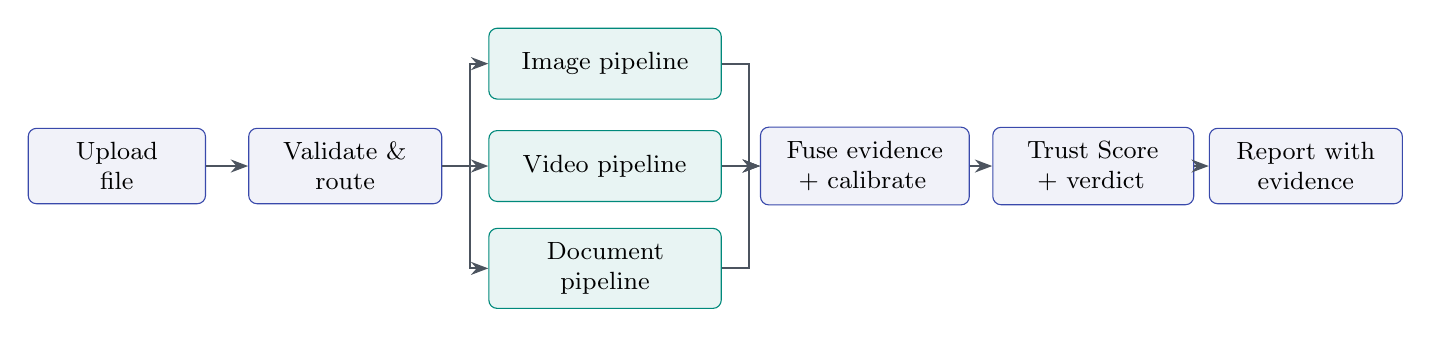
\begin{tikzpicture}
  \node[block, text width=1.9cm] (up) at (0,0) {Upload\\ file};
  \node[block, text width=2.1cm] (rt) at (2.9,0) {Validate \&\\ route};
  \node[ablock, text width=2.6cm] (im) at (6.2,1.3) {Image pipeline};
  \node[ablock, text width=2.6cm] (vi) at (6.2,0) {Video pipeline};
  \node[ablock, text width=2.6cm] (dc) at (6.2,-1.3) {Document pipeline};
  \node[block, text width=2.3cm] (fu) at (9.5,0) {Fuse evidence\\ + calibrate};
  \node[block, text width=2.2cm] (ts) at (12.4,0) {Trust Score\\ + verdict};
  \node[block, text width=2.1cm] (rp) at (15.1,0) {Report with\\ evidence};
  \draw[flow] (up) -- (rt);
  \draw[flow] (rt.east) -- ++(0.35,0) |- (im.west);
  \draw[flow] (rt) -- (vi);
  \draw[flow] (rt.east) -- ++(0.35,0) |- (dc.west);
  \draw[flow] (im.east) -- ++(0.35,0) |- (fu.west);
  \draw[flow] (vi) -- (fu);
  \draw[flow] (dc.east) -- ++(0.35,0) |- (fu.west);
  \draw[flow] (fu) -- (ts);
  \draw[flow] (ts) -- (rp);
\end{tikzpicture}
\end{adjustbox}
\caption{How the system works.}
\end{figure}

% =====================================================================
\section{Algorithms at a glance}

\begin{center}
\footnotesize
\begin{tabularx}{\linewidth}{@{}>{\raggedright\arraybackslash}p{2.3cm} >{\raggedright\arraybackslash}p{4.1cm} Y@{}}
\toprule
\textbf{Step} & \textbf{Algorithm} & \textbf{Why we use it} \\
\midrule
\multicolumn{3}{@{}l}{\textbf{\color{cPrimary}Phase 1 --- Image}} \\
Preprocessing & Same-format re-encoding, center crop $224{\times}224$ & Stops the model from learning ``JPEG = real'' shortcuts; cropping keeps fine artifacts that resizing would blur \\
Semantic features & \textbf{CLIP ViT-L/14} image encoder (frozen) & General features from 400M images; generalizes to unseen generators \\
Forensic features & \textbf{FFT} of the noise residual, radial spectrum (64 values) & Generators' up-sampling leaves periodic frequency traces \\
Classifier & \textbf{Logistic regression} head & Simple, fast, cannot over-fit to one generator \\
Baseline & \textbf{EfficientNet-B0} with transfer learning & Standard CNN to compare against \\
Explanation & \textbf{Grad-CAM}, patch score map, spectrum plot & Shows where and why the image looks AI-generated \\
Calibration & \textbf{Platt / temperature scaling} & Makes ``80\%'' mean 80\% \\
\midrule
\multicolumn{3}{@{}l}{\textbf{\color{cPrimary}Phase 2 --- Video}} \\
Frame sampling & 1 frame per second, max 32 & Keeps processing time small \\
Face detection & \textbf{MTCNN} (P-Net, R-Net, O-Net cascade) & Finds and aligns faces, where face-swaps happen \\
Frame classifier & CLIP features + logistic regression & Same generalizing design as Phase 1 \\
Aggregation & \textbf{Top-$k$ mean} of frame scores & Catches short fake segments without being noisy \\
\midrule
\multicolumn{3}{@{}l}{\textbf{\color{cPrimary}Phase 3 --- Document}} \\
Text reading & \textbf{OCR} (Tesseract LSTM / EasyOCR) & Words and their positions for checks and highlighting \\
Forensic maps & \textbf{ELA}, \textbf{SRM} noise filters, \textbf{DCT} coefficients & Edited regions have different compression and noise \\
Localization & \textbf{Dual-stream U-Net}, loss = BCE + Dice & Outputs a pixel mask of edited regions \\
Training data & Synthetic forgery generator (copy-move, splice, re-typed text) & Exact ground-truth masks without waiting for datasets \\
Logic checks & Arithmetic check, date check, \textbf{modified z-score} font check & Catches forgeries that are pixel-perfect but logically wrong \\
PDF checks & Structure analysis (incremental updates, dates, fonts) & Edited PDFs leave traces in the file itself \\
\midrule
\multicolumn{3}{@{}l}{\textbf{\color{cPrimary}Trust Scoring Engine (all phases)}} \\
Fusion & \textbf{Logistic regression} over all evidence & Weights show which evidence mattered \\
Score & $T=\operatorname{round}(100(1-p_{\text{manip}}))$ & One comparable score for all content types \\
Verdict bands & \textbf{Selective classification} thresholds & Unsure cases go to human review instead of a wrong answer \\
Explanation & Evidence-filled templates & Plain language that never claims more than was measured \\
\bottomrule
\end{tabularx}
\end{center}

% =====================================================================
\section{How the main algorithms work}

\subsection*{CLIP features (Phase 1 and 2)}
CLIP is a vision transformer trained on about 400 million image--text pairs. We pass the image
through it once and keep the 768-number output vector, normalized to length 1:
$\mathbf{z}=g(x)/\lVert g(x)\rVert$. The encoder is \emph{frozen} (not retrained), so it cannot
memorize one generator's quirks; this is why it generalizes to unseen generators (Ojha et al., CVPR 2023).

\subsection*{Frequency features (Phase 1)}
We remove image content with a median filter to keep only fine noise, $r=Y-\operatorname{Med}_{3\times3}(Y)$,
take its 2-D Fourier transform, and average the log-magnitude spectrum over 64 rings around the
center. AI up-sampling produces periodic peaks in this spectrum that real camera photos do not have.

\subsection*{Classifier and calibration}
The two feature vectors are joined and scored by logistic regression,
$\ell=\mathbf{w}^{\top}[\mathbf{z};\boldsymbol{\phi}]+b$, trained with binary cross-entropy. The score is then
calibrated on validation data, $p=\sigma(a\ell+c)$, so that the probability can be trusted.

\subsection*{Grad-CAM (explanation)}
Grad-CAM weights the last convolutional feature maps $A^k$ by the average gradient of the class score $y$:
\[
  L=\operatorname{ReLU}\Bigl(\sum_k\alpha_k A^k\Bigr),\qquad \alpha_k=\frac{1}{Z}\sum_{i,j}\frac{\partial y}{\partial A^k_{ij}} .
\]
The result is a heatmap of the regions that drove the decision.

\subsection*{MTCNN and temporal aggregation (Phase 2)}
MTCNN finds faces with three small CNNs in a cascade (propose, refine, output box and 5 landmarks).
Each face crop gets a probability $p_t$; the video score is the mean of the top 20\% of frame scores,
so a short manipulated segment is not averaged away.

\subsection*{ELA, SRM and DCT (Phase 3)}
\textbf{ELA} re-saves a JPEG and looks at the difference $\lvert x-J_{90}(x)\rvert$: edited regions react
differently. \textbf{SRM} filters are fixed high-pass kernels that expose noise patterns where text was
pasted or re-typed. \textbf{DCT} coefficients of $8{\times}8$ JPEG blocks reveal regions with a different
compression history.

\subsection*{Dual-stream U-Net (Phase 3)}
A U-Net is an encoder--decoder network with skip connections that outputs a mask the size of the
page. One encoder reads the RGB page; a second reads the SRM/ELA/DCT maps; the decoder combines both.
Because edited pixels are rare, the loss adds Dice to cross-entropy:
$\mathcal{L}=\mathcal{L}_{\text{BCE}}+1-\frac{2\sum\hat M M}{\sum\hat M+\sum M}$.

\subsection*{Trust Score and verdict}
All evidence (model score, frequency score, localization score, rule flags) forms a vector $\mathbf{e}$.
A logistic model gives $p_{\text{manip}}=\sigma(\boldsymbol\beta^{\top}\mathbf{e}+\beta_0)$ and
$T=\operatorname{round}(100(1-p_{\text{manip}}))$. Two thresholds, chosen on validation data so that
automatic decisions are wrong at most 5\% of the time, split $T$ into the three verdicts.

\subsection*{How accuracy is measured}
Separate train / validation / test sets; results always reported for \emph{seen} and \emph{unseen}
generators; metrics: accuracy, precision, recall, F1, AUC, pixel F1 and IoU (documents), and
calibration error; robustness tests after JPEG compression, resizing and blur; comparison with the
EfficientNet-B0 baseline.

\vspace{1em}
\noindent{\small\color{cMuted}Full details (UML and DFD diagrams, flowcharts, pseudocode, references) are in the
\emph{System Design} document.\par}

\end{document}
